\documentclass[a4paper]{article}

\usepackage[english]{babel}
\usepackage[utf8x]{inputenc}
\usepackage{amsmath}
\usepackage{amsfonts}
\usepackage{graphicx}
\usepackage[colorinlistoftodos]{todonotes}
\usepackage{makecell}

\title{CS 5785 -- Applied Machine Learning -- Lec.\ 1}
\author{Prof.\ Nathan Kallus, Cornell Tech
\\Scribe: TBD}
\date{August 23, 2018}

\begin{document}
\maketitle


\section{Logistics}

\begin{itemize}
\item Welcome!
\item Introduce TA: Andrew Bennett (office hours: TBD).
\item Course website: {\tt https://cs5785-2018.github.io}
\item 4 Homeworks (each with written exercises, programming exercises)
\item Homework 0 (for configuring your programming environment) due: Sep.~5, 2018 9:30am
\item 1 prelim exam (in-class), 1 final exam (take-home)
\item Surprise in-class quizzes (to encourage attendance)
\item The officially supported programming language is Python (with the numpy and scikit-learn packages) but homework can be also be done MATLAB (cheap student version at Cornell Store), R or Octave.
\item Required Textbook: Hastie, Tibshirani and Friedman (HTF) 3/e (available online, free): http://statweb.stanford.edu/$\sim$tibs/ElemStatLearn/
\item Assorted recommended textbooks: Murphy, Harrington, Rajaraman, Bishop, $\ldots$
\item Kaggle (https://www.kaggle.com/) is also a recommended website that holds leaderboards for different Machine Learning algorithms
\item See website for grading breakdown and homework submission instructions via CMS.
\item Collaboration encouraged, proper citation of references/sources is a must.
\item Guest lectures from researchers and practitioners in academia and industry.
\item Slack: https://cs5785-2018fa-kallus.slack.com 

\end{itemize}

\section{What is Applied Machine Learning?}
% Unpack the title:
% \begin{itemize}
% \item \emph{Analytics} is essentially ``counting stuff,'' or ``asking questions where the answer is something you can count.'' (H.\ Mason)
% \item \emph{Modern} refers to some combination of the following: predictive, statistical, machine learning based, big data. It is where analytics gets intersected with probability and machine learning.
% \end{itemize}
Applied Machine Learning is somewhere between Theoretical Machine Learning and Data Science.
Data Science has emerged as a hot area in the last few years.  What is a data scientist?  Tongue-in-cheek answer: ``person who is better at statistics than any software engineer and better at software engineering than any statistician.'' (J.\ Wills)

We need to be aware of statistics vs.\ ``punk stats.''  In punk music, you can still make songs even though you only know three chords. And in \ ``punk stats'' you can sometimes get a lot done even if you are not exercising real statistical methods and discipline. The best musicians know all the rules and then go about breaking them: same for this stuff.  Example of ``punk stats'': confusing population mean $\mu$ with sample mean $\bar x$.

Examples of applied machine learning in use today:
\begin{itemize}
\item Uber: app for car service
\item Google AdSense: content driven advertising
\item Waze: GPS w/traffic updates
\item Retail Shopping
\item Public Health
\item Netflix: movie recommendation
\end{itemize}
What are some examples you know of companies that use ``big data'' for Machine Learning?  ``The Unreasonable Effectiveness of Data'' by Halevy et al.\ (2009) summarizes some of the data driven approaches behind Google's recent breakthroughs in language translation and speech recognition.

Kaggle is a popular website where (aspiring) data scientists tackle ``challenge problems.''  Good way to get a sense for what works in practice.  We'll use some datasets posted there in this class.


\section{Lazy Learning}
``Lazy Learning'' stands in contrast to ``Eager Learning''. Data driven approaches may not yield deep insights, but they can be very powerful.  In so-called ``lazy learning'' approaches we don't need to fit a model, just store examples.  They're memory based -- just store lots of labeled examples (for example, a big collection of 28$\times$28 images of handwritten digits). When an unknown digit image comes in, you compare it to all of the stored values, supply a distance function and return a label based on nearest neighbor(s).  This is in contrast to ``eager learning,'' in which we try to \emph{generalize} from training data.

As an example of ``lazy learning,'' imagine that you are building a handwriting recognizer. The ``lazy learning" approach might be to collect lots of examples of handwritten letters and store them in a huge array. Then, when you want to classify new instances that come along, you simply compare all the examples stored in memory to everything in the array. (Yes, as you might imagine, this is wasteful approach; but remember that storage is cheap; so, don't always dismiss this approach outright)

Important distinction: \emph{training} data vs.\ \emph{testing data}.  One should never mix these. What is the difference between testing and training data? Testing data is \textbf{sequestered}, and put aside to evaluate something you have trained. Training data is data you give to your computer to build the learning. Sites like Kaggle often sequester an evaluation set, revealing only at the moment of competition.  Otherwise the entrants would have trouble resisting the urge to iterate running their algorithms on training data, evaluating them on testing data, tweaking parameters and -- inevitably -- overfitting to a finite sample of the data.  Later we'll study a method called \emph{cross validation} that will help us avoid overfitting.

\subsection{$k$-Nearest Neighbor}

$k$-nearest neighbor (kNN), where $k$ is usually a small integer, is the most popular example of a ``lazy learning'' approach [HTF \S 13.3].  It's one of the baseline algorithms on Kaggle.  The task for kNN is to predict class $Y \in G$ based on observation $X$. Some examples for possible $G$ and $X$ include: $G=\{-1,1\}, \{ \text{high risk, low risk, no risk}\}, X=28^2$ real numbers between 0 and 1. Given a new query $x_0$, kNN does the following:
\begin{itemize}
\item Find the $k$ training points.\ $x_{(r)}$, $r=1,\ldots,k$ closest in distance to $x_0$.
\item Classify $x_0$ using majority vote among the $k$ neighbors:
   
$\hat{Y}=\underset{g\in G}{\operatorname{argmax}} \sum_{i=1}^{k} 1[y_i=g]$
\item Break ties at random (more relevant for multiple classifier situations that allow for ties).
\end{itemize}

This requires us to have a distance measure. Let $x$ be a vector of features (real numbers). 

$x = \left[ \begin{array}{ccc} x_1\\ \vdots\\ x_p\\ \end{array} \right] \in \mathbb{R}^p$
   
Simple example of a distance function is Euclidean distance:

$||x-x'||_2 = \sqrt{\sum_{j=1}^{p} (x_j - x'_j)^2}$

We are going to compute its distance to all saved training examples. The distance function captures the quantitative notion of similarity.

Note: query pt.\ $x_0$ can be any ``feature vector.'' For example, if height and weight are your two features, the \emph{column vector} $x_0$ might be
$$x_0 = \left[\begin{matrix} h_0 \\ w_0 \end{matrix} \right]$$
where $h_0$, $w_0$ are the height and weight of the query item respectively. In the example of the handwritten digit, you may have a feature vector 784 dimensions long each representing pixel brightness. When calculating distance, you would line up the two feature vectors subtract every entry for $x_0$ from every entry of the neighbor, square every difference, and add them all up. This is your distance.

Note: we often \emph{standardize} the feature to have mean 0 and variance 1 across all the points in the dataset.  Otherwise, certain features can impact the distance disproportionately, as when measurements are done with wildly varying units such as ounces vs.\ tons. Example: The above feature vector might set $h_0$ to have units of meters and $w_0$ may have units of pounds. What would distance mean within this space? Standardization makes this less necessary. Other methods for standardize the vector data includes making each component have mean 0 and unit covariance or scaling so that max $=1$ and min $=-1$. 

How do we choose $k$?  This is an instance of \emph{model order selection}.  In general it is a very hard problem in machine learning, a special case of \emph{model selection}.  But one popular method for choosing $k$ is to use \emph{cross validation} [HTF \S 7.10].
To cross validate your data, first pick some arbitrary number of folds $N$ and an initial guess of $k$. 
% $k$ typically ranges in value from 5-15, commonly (5,7,9), and usually takes on an odd value.  
Then, divide up your data into $N$ ``buckets.'' As you do so, label one of the buckets as your test data and the others as your training data. Create your model and test it. Then, rotate the buckets, so a new one is the testing bucket, and do it all over. Do this until every bucket has served as the testing bucket. Once that is done, change your $k$ and do the whole process over. If you do this across a range of set a $k$ values, it might help you select an optimal $k$. See Table \ref{tab:crossval} for an illustration of $N$-fold cross validation using $N=5$ buckets.

\begin{table}
\small
\centering
\begin{tabular}{|
>{\centering\arraybackslash}p{0.125\textwidth}|
>{\centering\arraybackslash}p{0.7cm}|
>{\centering\arraybackslash}p{1.35cm}|
>{\centering\arraybackslash}p{1.35cm}|
>{\centering\arraybackslash}p{1.35cm}|
>{\centering\arraybackslash}p{1.35cm}|
>{\centering\arraybackslash}p{1.35cm}|}
\hline
Side Iter & \makecell{Iter\textbackslash \\ Fold} &1 & 2 & 3 & 4 & 5\\ \hline
\makecell{k=5, k=7, \\ k=9,...} & 1 & Validation & Train & Train & Train & Train\\ \hline
\makecell{k=5, k=7, \\ k=9,...} & 1 & Train & Validation & Train & Train & Train\\ \hline
\makecell{k=5, k=7, \\ k=9,...} & 1 & Train & Train & Validation & Train & Train\\ \hline
\makecell{k=5, k=7, \\ k=9,...} & 1 & Train & Train & Train & Validation & Train\\ \hline
\makecell{k=5, k=7, \\ k=9,...} & 1 & Train & Train & Train & Train & Validation\\ \hline
\end{tabular}
\caption{\label{tab:crossval}Illustration of 5-fold cross validation. Fit on the training folds, measure prediction on the validation fold.}
\end{table}
Step through each fold for validation, measure the mean and variance of the error.  This prevents you from getting to attached to any one subset of data and thus \emph{overfitting}.

Cross validation is useful for \emph{parameter selection}. If you wish to pick an appropriate $k$ to use in kNN, for example, you can try a range of values for $k$ (e.g., $1,\ldots,15$), use $N$-fold cross validation to pick the $k$ that maximizes average validation accuracy.

\section{Supervised Learning}
In addition to being an instance of lazy learning, kNN is also an example of \emph{supervised learning}. In a supervised learning scenario, each observation has a \emph{feature vector} and a categorical \emph{label} that is known \emph{a priori} for every point. This is in contrast to \emph{unsupervised learning}, where the data has no labels and you can only draw conclusions about the \emph{distribution} of the data.

Two main categories of supervised learning are classification and regression.  We'll get to regression later.

Example: 2-class classification [HTF \S 2.4].  We have an input vector $X\in \mathbb{R}^p$ with outcome variable $Y\in\{-1,1\}$. This label could be male/female, yes/no, for example.  We use $(x_i,y_i)$ to denote our $p+1$ dimensional training observations.  The extra dimension comes from tacking the outcome variable to the end of each vector.

Now put aside kNN for a moment and consider the question, in general, how well can we hope to do on this classification task?

\subsection{Bayes Error Rate}
This is the same Bayes as the Rev.\ Thomas Bayes, famous for the theorem that bears his name:
$$P(B|A) = \frac{P(B)P(A|B)}{P(A)}$$
Let $G$ denote the \emph{categorical} output class variable and $\hat G$ our estimate of it.  $\hat G$ assumes values in $\mathcal G$, the set of $K$ possible classes, which is $2$ in this case.  Using $\mathcal G$ is more general than the \emph{quantitative output} form of $Y=\{-1,1\}$ above.

In order to quantify how well we're doing, we need to define a \emph{loss function}, represented by a $K\times K$ matrix $L$, with $K=card(\mathcal{G})$, the cardinality of $\mathcal G$.

\begin{itemize}
\item Examples of categorical output variables: A binary classifier might output one of $\{\textsc{Yes}, \textsc{No}\}$, $\{\textsc{Male}, \textsc{Female}\}$, $\{0, 1\}$, or $\{-1, +1\}$, and so on. The ``Ivy League'' 8-class classifier might select a label from the set
$\{\textsc{Brown},$ $\textsc{Columbia},$ $\textsc{Cornell},$ $\textsc{Dartmouth},$ $\textsc{Harvard},$ $\textsc{UPenn},$ $\textsc{Princeton},$ $\textsc{Yale}\}$.
\item $L$ is 0 on the diagonal and nonnegative elsewhere
\item $L(k,l)$ tells us the price paid for classifying an observation belonging to class $\mathcal{G}_k$ as $\mathcal{G}_l$
\item Example: we pay some cost for misclassifying an apple as an orange, and perhaps a lower cost for misclassifying an apple as a pear.
\item Example: \emph{zero-one} loss function, where $L$ looks like the opposite of an identity matrix
\end{itemize}

Now we can ask, what is the expected prediction error?  We write this as
$$EPE=E[L(G,{\hat G}(X))]$$
L is a look up table and the expected value is computing a weighted average.
We seek to minimize the prediction error and we are going to compute the expectation w.r.t. the joint distribution, expressed using the chain rule of probability:
$$ Pr(G, X) = Pr (G | X) P(X)$$
The probability of G, given X times the probability of X.
We compute the expectation w.r.t.\ the joint distribution $\text{Pr}(G,X)$:
$$EPE=E_X\sum_{k=1}^K L[\mathcal{G}_k,{\hat G}]\text{Pr}(\mathcal{G}_k|X)$$
Here we are summing over the $K$ possible classes; we have the loss function.\ weighted by $\text{Pr}(G,X)$ where we've conditioned on $X$, i.e., $\text{Pr}(G,X)=\text{Pr}(G|X)\text{Pr}(X)$.

We want to find the $\hat G$ that minimizes EPE; it suffices to minimize it pointwise:
$${\hat G}(x) = \arg \min_{g\in\mathcal{G}}\sum_{k=1}^K L(\mathcal{G}_k,g)\text{Pr}(\mathcal{G}_k|X=x)$$
If we plug in the 0-1 loss function, this becomes:
$${\hat G}(x) = \arg \min_{g\in\mathcal{G}}[1-\text{Pr}(g|X=x)]$$
which tells us that ${\hat G}(X)=\mathcal{G}_k$ if $\text{Pr}(\mathcal{G}_k|X=x)=\max_{g\in\mathcal{G}}\text{Pr}(g|X=x)$.
This is called the \emph{Bayes classifier}: it says classify to the most probable class, using the conditional distribution $\text{Pr}(G|X)$.  The error rate of this classifier is called the \emph{Bayes rate}.

HTF Fig.\ 2.5 shows a 2D example where the generating density is known for each class (Gaussian, in this case).

\begin{figure}
\centering
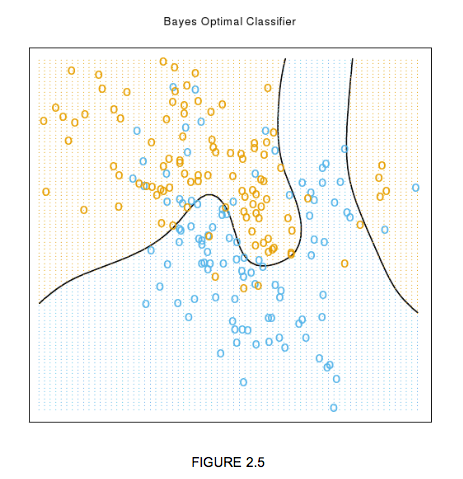
\includegraphics[width=0.75\textwidth]{HTFfig2_5.png}
%\caption{\label{fig:frog}HTF Fig.\ 2.5.}
\end{figure}

Note: take care not to confuse the \emph{Bayes rate} with the \emph{base rate}.  The base rate is what you get simply by picking the most frequent class in your training data.  This is a good reality check to try before pursuing complicated solutions.

The \emph{Bayes rate} is the best possible error rate of any classifier (over the distribution of all samples, for the chosen hypothesis space).

How do we connect this back to the kNN classifier?  The kNN classifier directly approximates this solution using a majority vote in a neighborhood, probabilities estimated by training-sample proportions.  This is shown in HTF Fig.\ 2.2. Note that Bayes is not an alternative to kNN; think of Bayes more as the theoretically perfect model you try to approach or approximate using kNN.

\begin{figure}
\centering
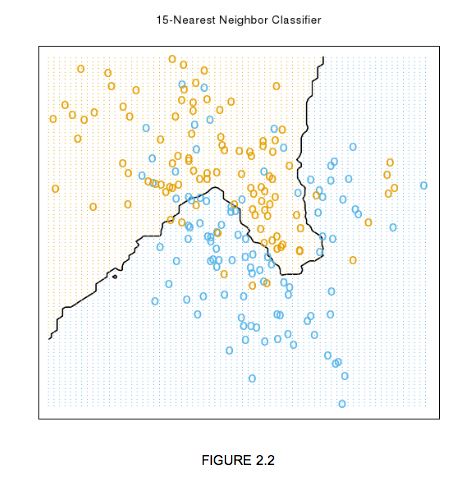
\includegraphics[width=0.75\textwidth]{HTFfig2_2.png}
\end{figure}


One can also use the binary $Y=\{-1,1\}$ and squared error loss to arrive at the same result.  We leave this as an exercise.

Whenever using nearest neighbor methods, we need to be aware of the \emph{curse of dimensionality}.  We're return to that topic later.



\end{document}	
